\graphicspath{{content/chapters/3_literature/figures/}}
\chapter{Literature Review}
\label{sec:literature_review}

This chapter presents an overview of relevant machine learning methods used for speech enhancement, with particular emphasis on the autoencoder architecture. It begins by introducing the fundamental principles behind neural networks and their biological inspiration, followed by a detailed discussion of machine learning techniques applied to noise suppression. Recent architectural advancements and training strategies are covered, culminating in the evaluation metrics used throughout this project to benchmark both classical and machine learning approaches.


\section{Neural Networks}
\label{sec:neural_networks}

Machine learning models, particularly neural networks, have been widely adopted for noise cancellation. Neural networks, inspired by biological neurons in the human brain, are composed of layers of interconnected processing units known as \textit{neurons}. Each artificial neuron receives multiple inputs, performs a weighted summation, applies a bias, and passes the result through an activation function to produce its output.

This structure draws direct inspiration from the way biological neurons function—where dendrites receive signals, the cell body processes them, and the axon transmits the signal to the next neuron. Figure~\ref{fig:neuron_vs_ann} illustrates this analogy.

\begin{figure}[H]
    \centering
    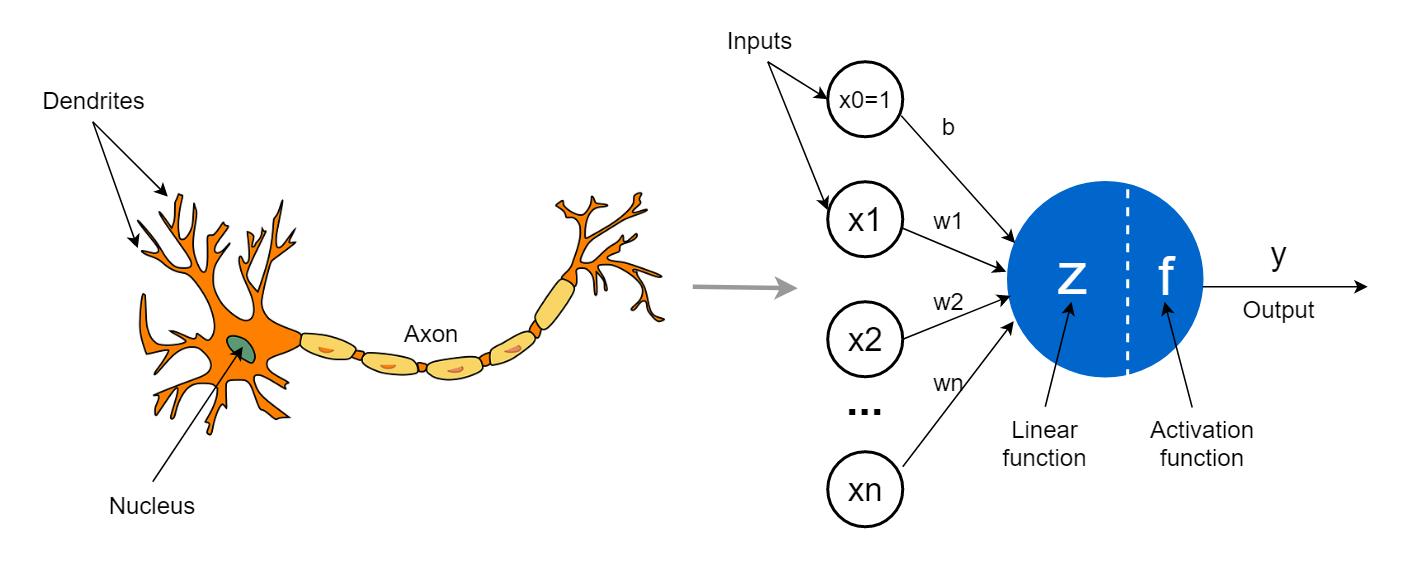
\includegraphics[width=0.75\textwidth]{neuron_vs_ann.png}
    \caption{Biological neuron vs. Artificial neuron structure.\cite{ghosh2020perceptron}}
    \label{fig:neuron_vs_ann}
\end{figure}

A typical neural network for noise cancellation consists of the following components:
\begin{itemize}
    \item \textbf{Input layer:} Receives the noisy speech signal (e.g., a time-domain waveform or its spectrogram).
    \item \textbf{Hidden layers:} Perform nonlinear transformations to extract key features and patterns from the input. These layers may include convolutional, recurrent, or fully connected neurons depending on the network architecture.
    \item \textbf{Output layer:} Produces the denoised speech signal by mapping the learned features back to the clean signal domain.
\end{itemize}

The network is trained using pairs of clean and noisy audio samples. It gradually learns to reduce the difference between its predicted output and the actual clean signal. Once trained, the model can take in new noisy speech and output a cleaner version. This learning-based approach allows neural networks to adapt to complex noise patterns, often performing better than traditional signal processing methods in real-world situations.

\section{Machine Learning}
\label{sec:machine_learning}

Machine learning (ML), a subset of artificial intelligence (AI), focuses on developing algorithms that enable systems to learn patterns from data and make decisions without being explicitly programmed. In speech enhancement, ML has enabled the design of specialised neural network architectures capable of recovering clean speech from noisy inputs. One widely used architecture is the \textit{autoencoder}, which learns to reconstruct its input via a compressed latent representation \cite{azarang2020review}.

\begin{figure}[h]
    \centering
    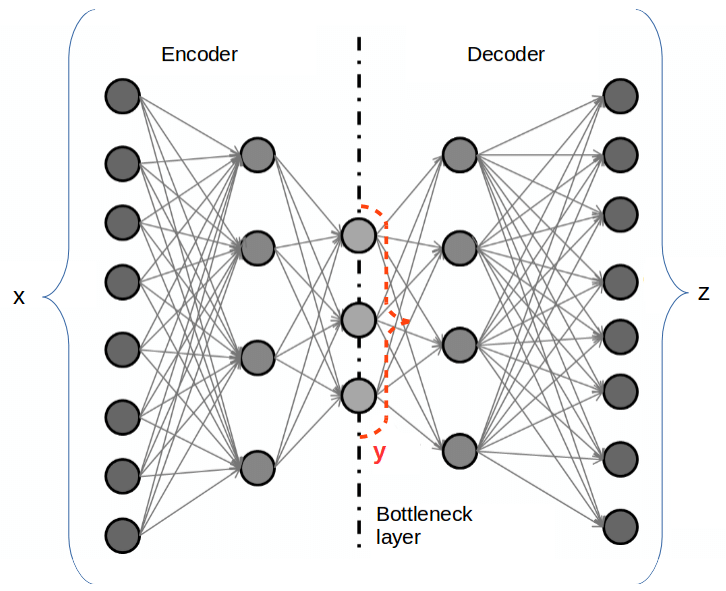
\includegraphics[width=0.5\textwidth,keepaspectratio]{autoencoder.png}
    \caption{\label{fig:autoencoder} Block diagram of an autoencoder architecture \cite{vachhani2017dae}.}
\end{figure}

An autoencoder consists of two main components: an encoder and a decoder. The encoder compresses the input signal \(x\) into a low-dimensional latent space by passing it through convolutional, pooling, or fully connected layers. A central \textit{bottleneck} layer enforces this compression, encouraging the model to retain only the most salient features—such as speech structure—while discarding irrelevant noise.

The decoder then reconstructs the signal \(y\) from the latent representation, typically using upsampling, transposed convolutions, or dense layers in a mirrored arrangement. The objective is to recover the clean speech with minimal reconstruction error.

Autoencoders are trained using paired datasets of noisy and clean speech. During training, the noisy input is passed through the network, and the output is compared to the clean reference. The model is optimised to minimise the difference—typically using a loss function such as Mean Squared Error (MSE) or Mean Absolute Error (MAE).

\begin{figure}[h]
    \centering
    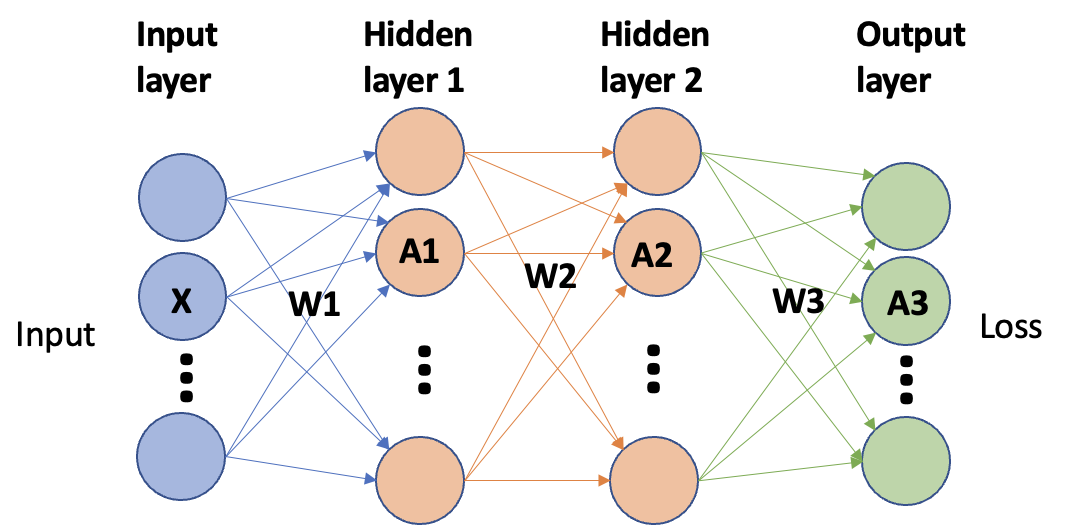
\includegraphics[width=0.5\textwidth,keepaspectratio]{weigths.png}
    \caption{\label{fig:weigths} Loss and weight update process in an autoencoder \cite{epoch2021}.}
\end{figure}

Training proceeds iteratively. A forward pass generates an output, and the loss function quantifies the error. This error is then propagated backward through the network via backpropagation to compute gradients, which are used to update the model’s weights using optimisers like Stochastic Gradient Descent (SGD) or Adam. This cycle continues for many epochs until convergence.

Recent advances have introduced more robust architectures. For example, Kim et al.~\cite{kim2024residual} proposed a residual-attention Gated Linear Unit (GLU) model for end-to-end (E2E) speech enhancement. Their model outperformed SOTA methods such as FAIR-Denoiser and CleanUNet across a wide SNR range (0–15 dB), showcasing the effectiveness of modern ML approaches.

Evaluation metrics such as SNR, PESQ, STOI, and MSE—used in these studies—will also be used in this project to assess and compare both classical and ML-based denoising systems. These metrics are discussed in detail in Chapter~\ref{chp:evaluation}.
